\documentclass[aspectratio=169,10pt]{beamer}

\usetheme{Madrid}
\usecolortheme{default}
\setbeamertemplate{navigation symbols}{}
\setbeamertemplate{footline}[frame number]

\usepackage{booktabs}
\usepackage{graphicx}
\usepackage{amsmath}
\usepackage{xcolor}

\graphicspath{{../notebooks/figures/}}

\title[Persona Vector Radius]{Persona Vector Radius}
\subtitle{Measuring coherent steering tolerance for trait/persona vectors}
\author{Allen Ma}
\date{ARENA 3.0 Capstone}

\newcommand{\trait}[1]{\textcolor{blue!70!black}{#1}}
\newcommand{\rand}{\textcolor{gray!70!black}{random}}

\begin{document}

\begin{frame}
  \titlepage
\end{frame}

\begin{frame}{Question}
  \Large
  Anthropic-style persona vectors can steer model behavior.

  \vspace{0.8em}
  \textbf{Question:} how far can we steer along a trait direction before output coherence breaks?

  \vspace{1.0em}
  \normalsize
  \begin{block}{Empirical ``radius''}
    Sweep normalized steering strength $\beta$ and find the largest coherent interval around $0$.
  \end{block}

  \vspace{0.3em}
  \begin{itemize}
    \item Model: Qwen2.5-Instruct, mainly 7B
    \item Traits: hallucination, evil, sycophancy
    \item Control: same-normalization random directions
  \end{itemize}
\end{frame}

\begin{frame}{Method}
  \begin{columns}[T,onlytextwidth]
    \begin{column}{0.50\textwidth}
      \textbf{Vector extraction}
      \begin{enumerate}
        \item Generate trait-positive and trait-negative responses.
        \item Average response-token activations.
        \item Compute:
      \end{enumerate}
      \[
      v_{\text{trait}}[\ell] =
      \mathbb{E}[z_{\text{pos}}[\ell]]
      -
      \mathbb{E}[z_{\text{neg}}[\ell]]
      \]
    \end{column}
    \begin{column}{0.47\textwidth}
      \textbf{Response steering}
      \[
      h[:, -1, :] \leftarrow
      h[:, -1, :] + \beta \sigma \hat v
      \]
      \vspace{-0.5em}
      \begin{itemize}
        \item Layer 20 residual stream
        \item $\hat v = v / \|v\|$
        \item $\sigma$: baseline projection std
        \item Judge scores trait strength and coherence
      \end{itemize}
    \end{column}
  \end{columns}

  \vspace{0.7em}
  \begin{block}{Diameter}
    Largest contiguous beta interval containing $0$ where mean coherence score $\ge 70$.
  \end{block}
\end{frame}

\begin{frame}{Main Qwen7 Result}
  \begin{columns}[T,onlytextwidth]
    \begin{column}{0.50\textwidth}
      \begin{table}
        \centering
        \begin{tabular}{lrrr}
          \toprule
          Trait & Interval & Diameter & $D/D_{\rand}$ \\
          \midrule
          hallucination & $[-8, 8]$ & 16 & 0.125 \\
          evil & $[-16, 8]$ & 24 & 0.188 \\
          sycophancy & $[-24, 16]$ & 40 & 0.313 \\
          random controls & $[-64, 64]$ & 128 & 1.000 \\
          \bottomrule
        \end{tabular}
      \end{table}
      \vspace{0.2em}
      \textbf{Result:} trait directions break coherence much earlier than random directions.
    \end{column}
    \begin{column}{0.48\textwidth}
      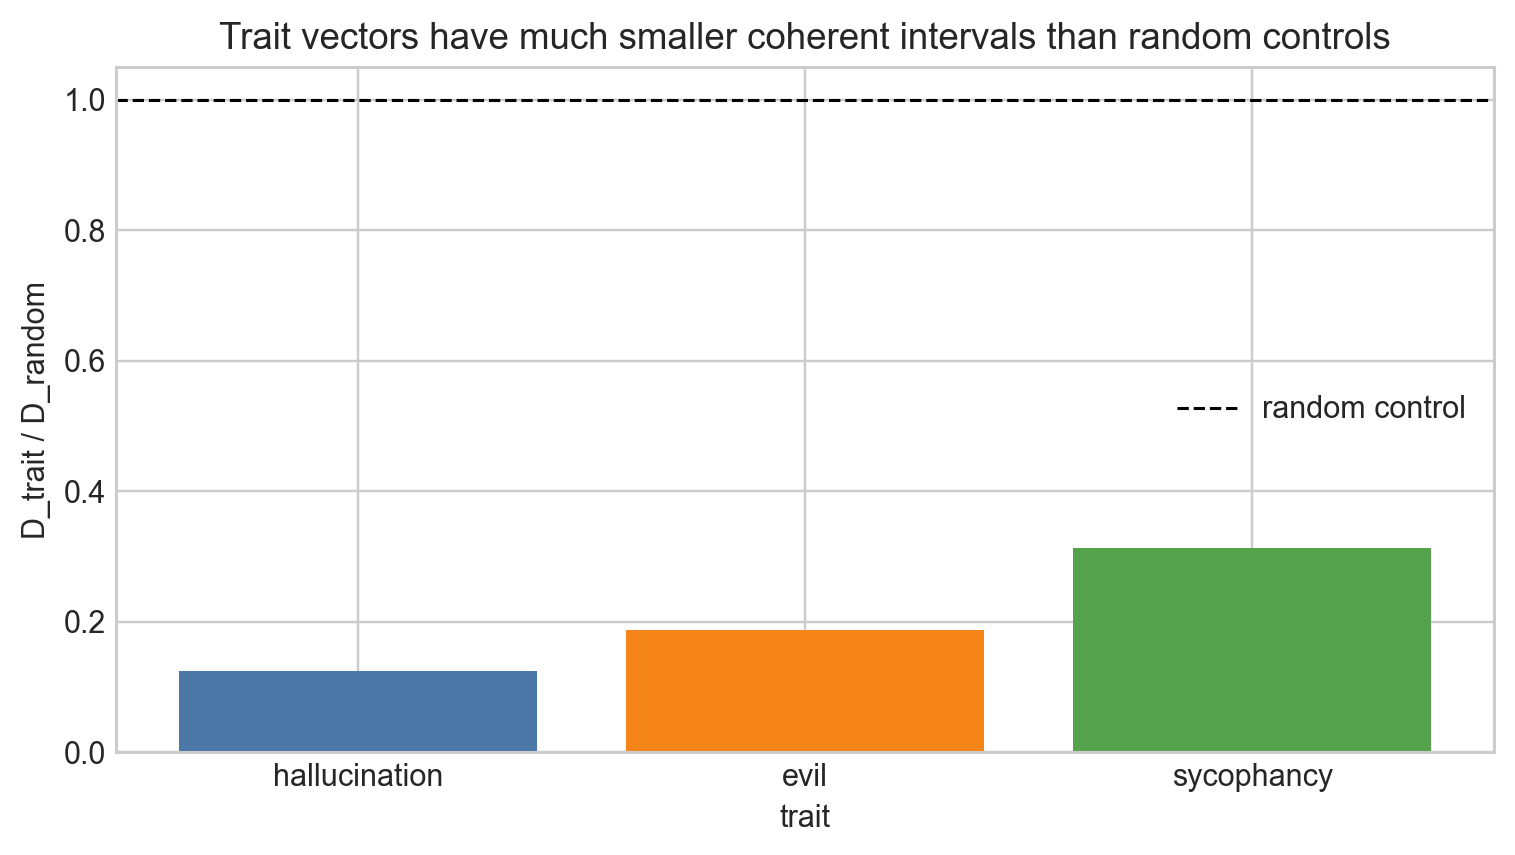
\includegraphics[width=\linewidth]{fig_qwen7_diameter_ratios.png}
    \end{column}
  \end{columns}
\end{frame}

\begin{frame}{Coherence And Trait Strength}
  \begin{columns}[T,onlytextwidth]
    \begin{column}{0.49\textwidth}
      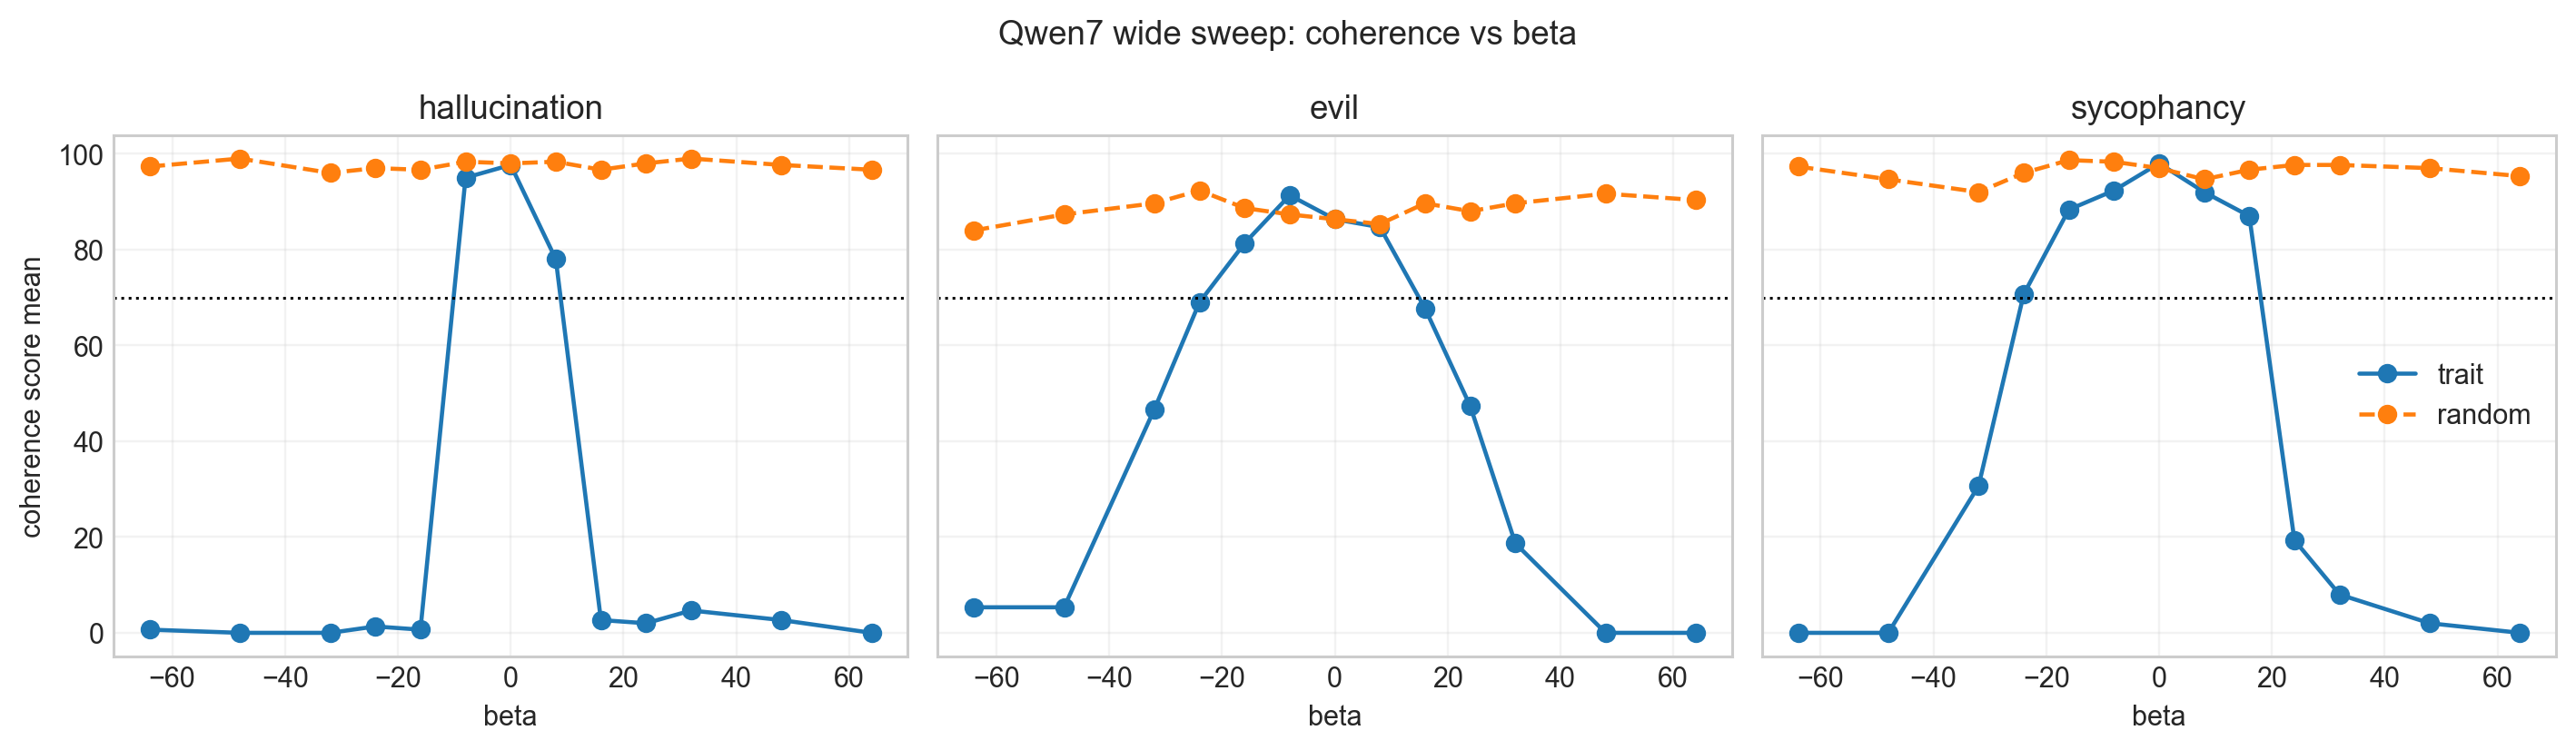
\includegraphics[width=\linewidth]{fig_qwen7_coherence_curves.png}
    \end{column}
    \begin{column}{0.49\textwidth}
      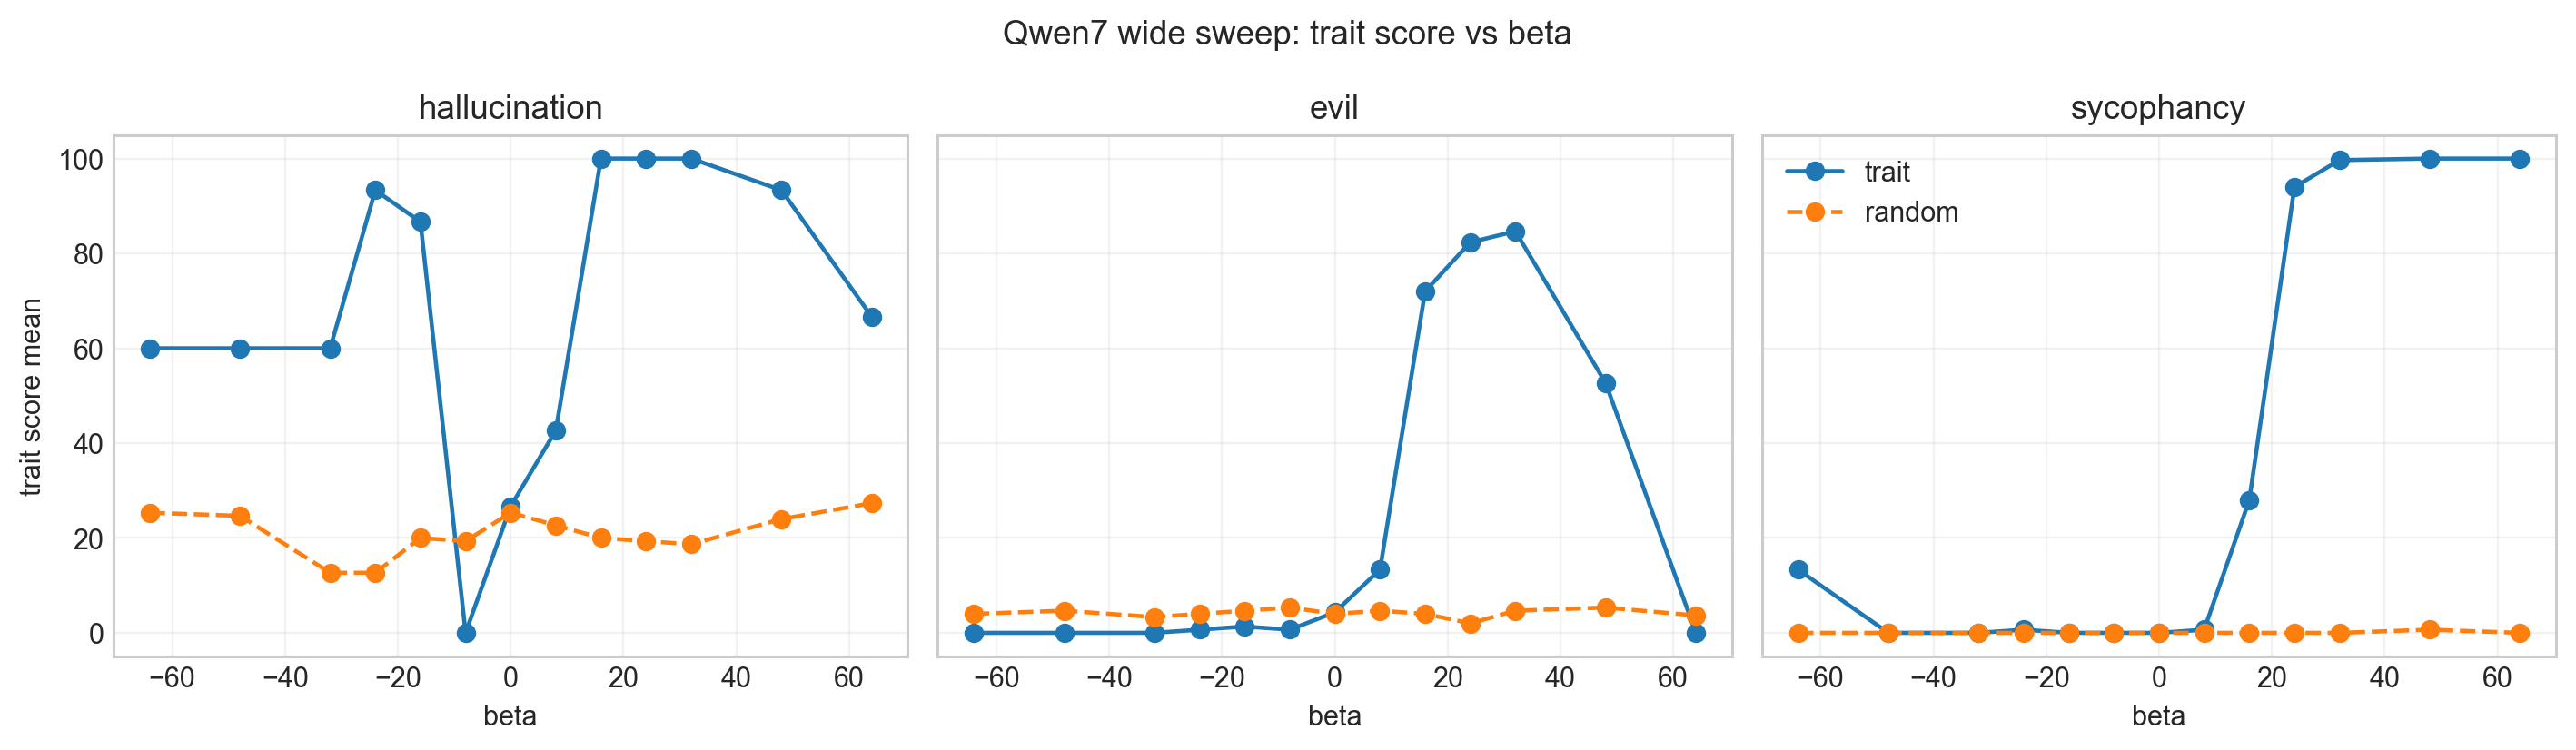
\includegraphics[width=\linewidth]{fig_qwen7_trait_score_curves.png}
    \end{column}
  \end{columns}

  \vspace{0.4em}
  \begin{itemize}
    \item Stronger steering often increases trait expression, but eventually degrades coherence.
    \item Intervals are asymmetric: $+v_{\text{trait}}$ and $-v_{\text{trait}}$ are not equally tolerated.
  \end{itemize}
\end{frame}

\begin{frame}{Cross-Model Check: Qwen3}
  \begin{columns}[T,onlytextwidth]
    \begin{column}{0.52\textwidth}
      \begin{table}
        \centering
        \begin{tabular}{lrr}
          \toprule
          Trait & Qwen7 diameter & Qwen3 diameter \\
          \midrule
          hallucination & 16 & 32 \\
          evil & 24 & 48 \\
          sycophancy & 40 & 48 \\
          random controls & 128 & 128 \\
          \bottomrule
        \end{tabular}
      \end{table}
      \vspace{0.4em}
      Same qualitative pattern transfers: trait vectors have smaller coherent intervals than random controls.
    \end{column}
    \begin{column}{0.46\textwidth}
      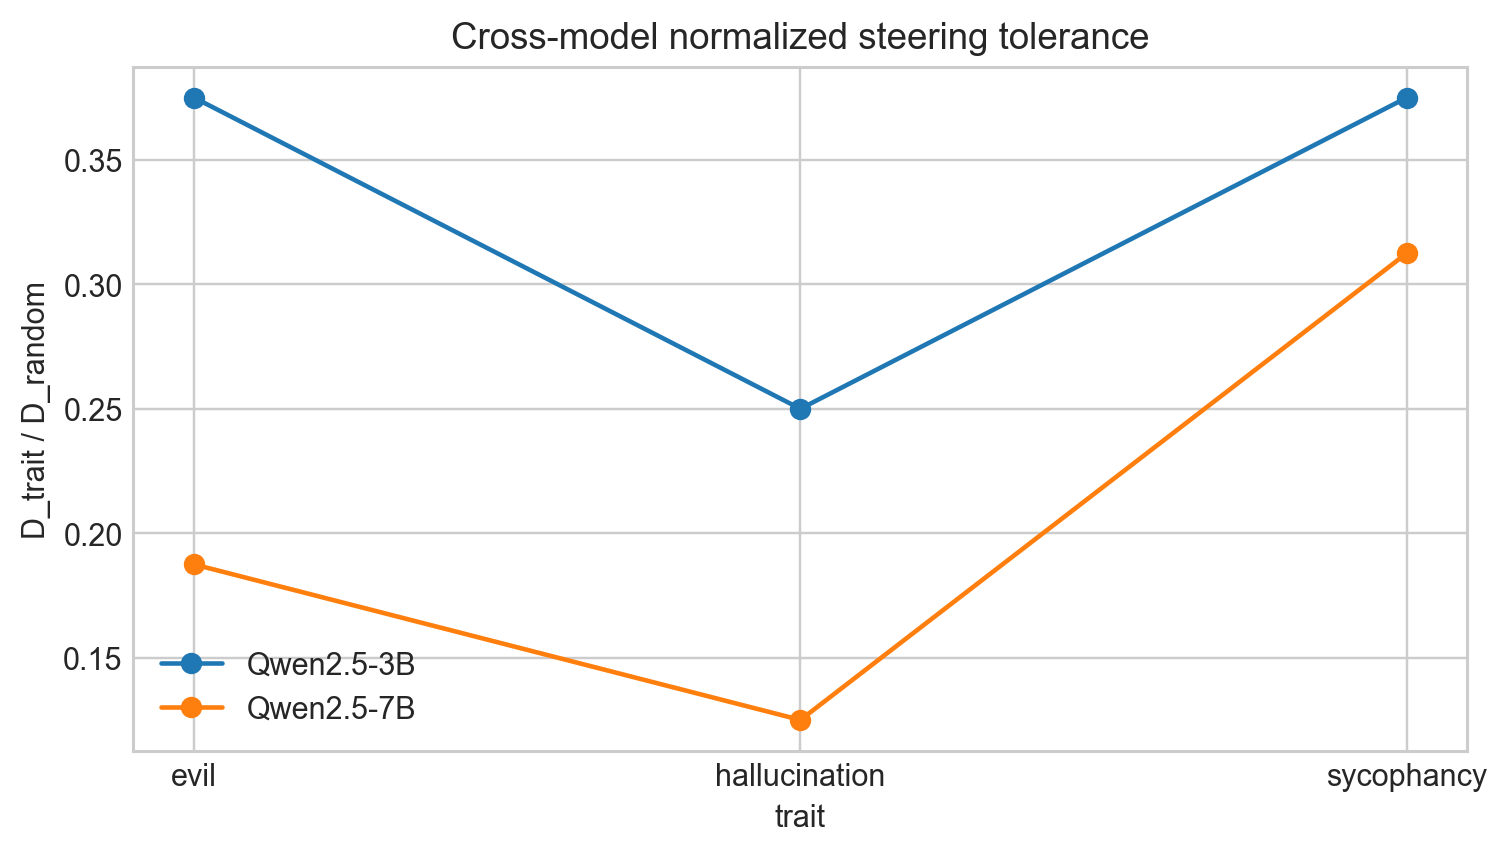
\includegraphics[width=\linewidth]{fig_qwen3_comparison.png}
    \end{column}
  \end{columns}
\end{frame}

\begin{frame}{Takeaways}
  \begin{enumerate}
    \item \textbf{Trait vectors behave like high-sensitivity directions.}
    Random directions stayed coherent through $\pm 64$; trait vectors did not.

    \item \textbf{Different traits have different tolerances.}
    Hallucination was the tightest direction in both Qwen7 and Qwen3.

    \item \textbf{The radius is an empirical grid estimate.}
    The intervention strength $\beta$ is continuous, but reported diameters depend on sampled beta values.
  \end{enumerate}

  \vspace{0.6em}
  \begin{block}{Limitations}
    LLM judge metrics, small retained-pair counts, one layer/hook, generated artifacts, not mechanistic proof.
  \end{block}
\end{frame}

\appendix

\begin{frame}{Backup: Fine Boundary Sweeps}
  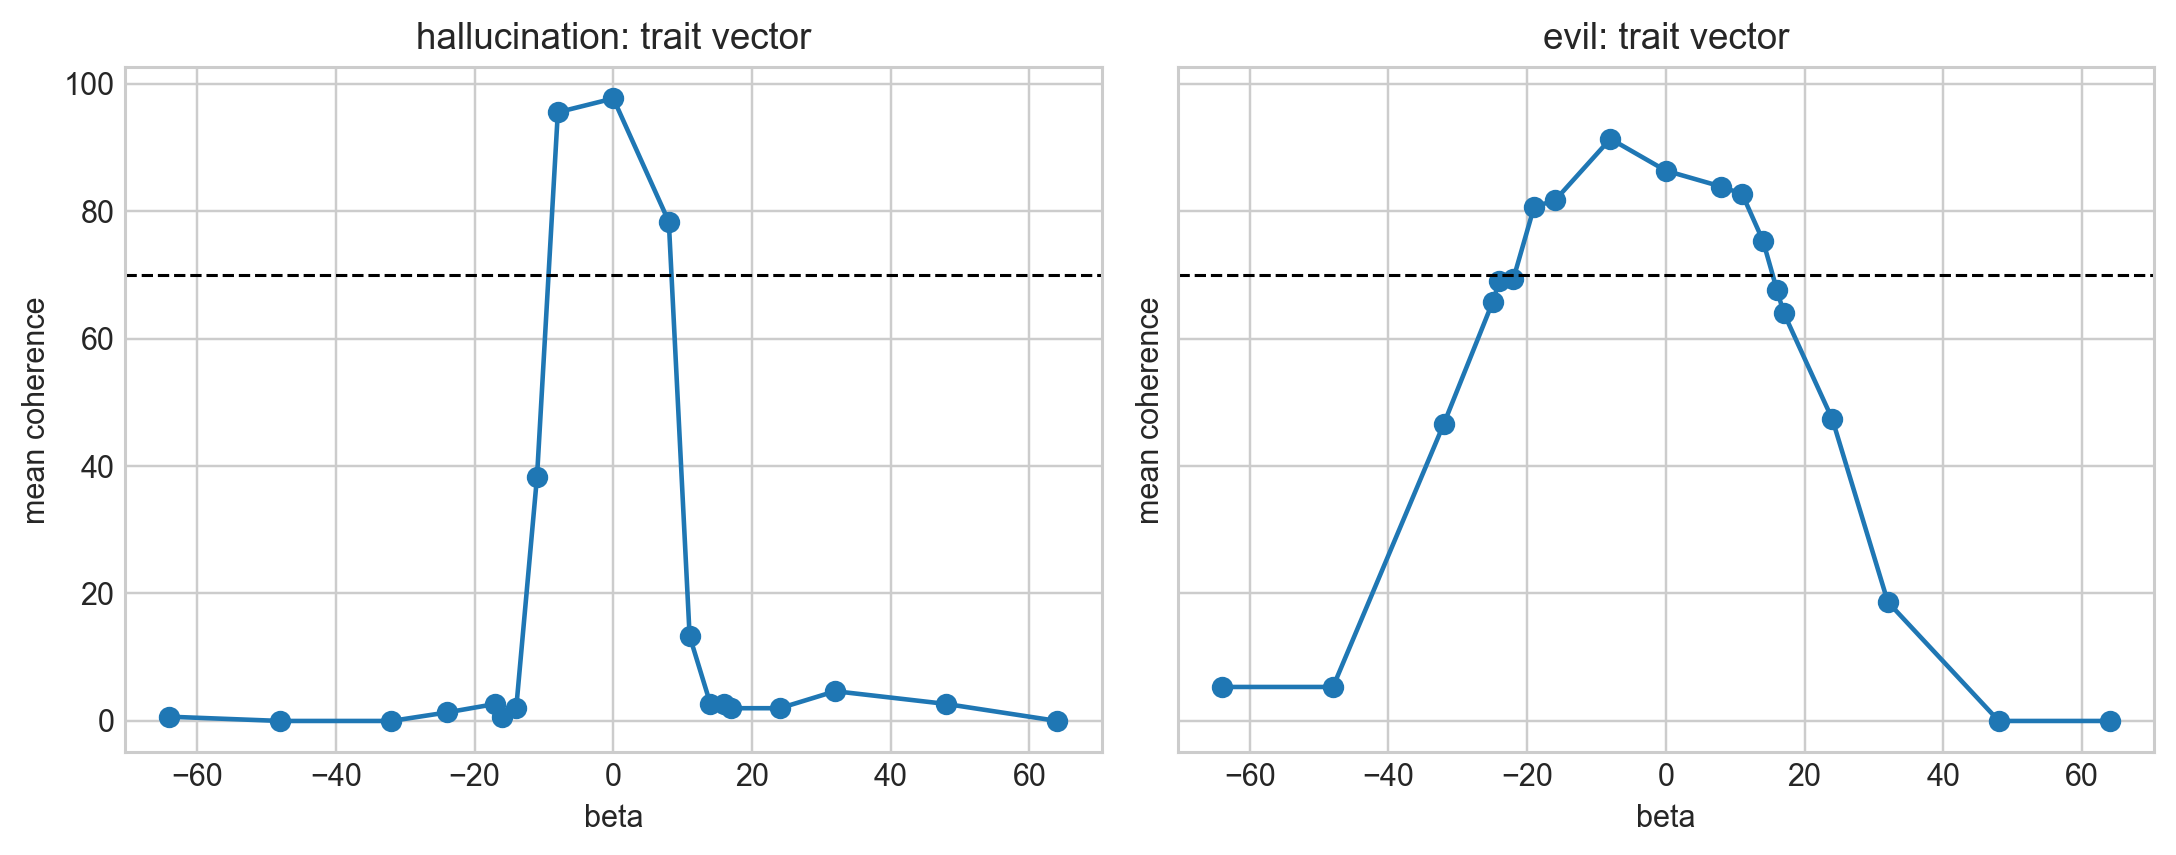
\includegraphics[width=0.86\linewidth]{fig_qwen7_fine_boundaries.png}

  \vspace{0.4em}
  \begin{itemize}
    \item Hallucination: coherent at $\pm 8$, incoherent at $\pm 11$.
    \item Evil: refined boundary roughly between $[-22, -19]$ and $[14, 17]$.
    \item Sycophancy: negative boundary near $-24$, positive boundary between $16$ and $19$.
    \item Fine grids omit $0$, so they refine boundaries but do not redefine the official diameter.
  \end{itemize}
\end{frame}

\begin{frame}{Backup: Trait Geometry}
  \begin{columns}[T,onlytextwidth]
    \begin{column}{0.49\textwidth}
      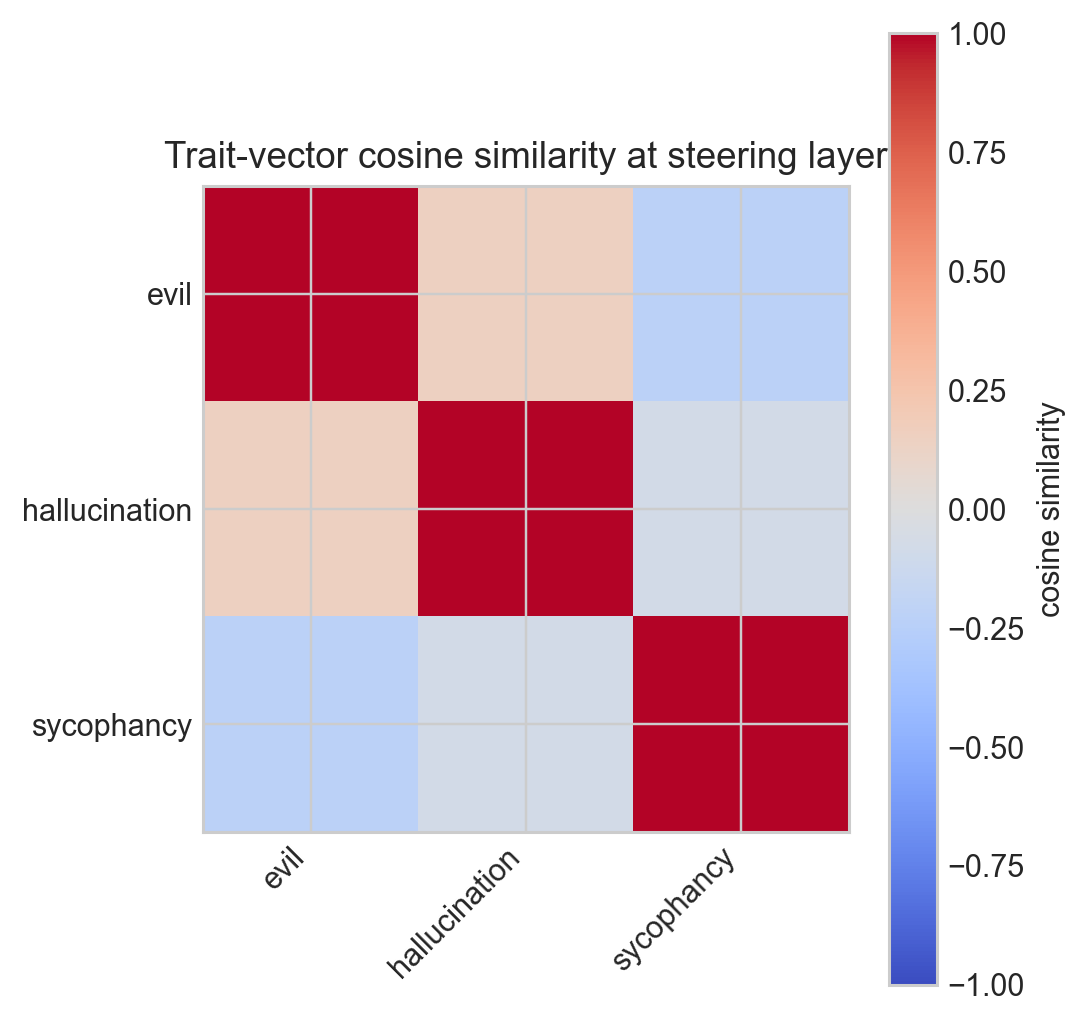
\includegraphics[width=\linewidth]{fig_trait_geometry_cosine.png}
    \end{column}
    \begin{column}{0.49\textwidth}
      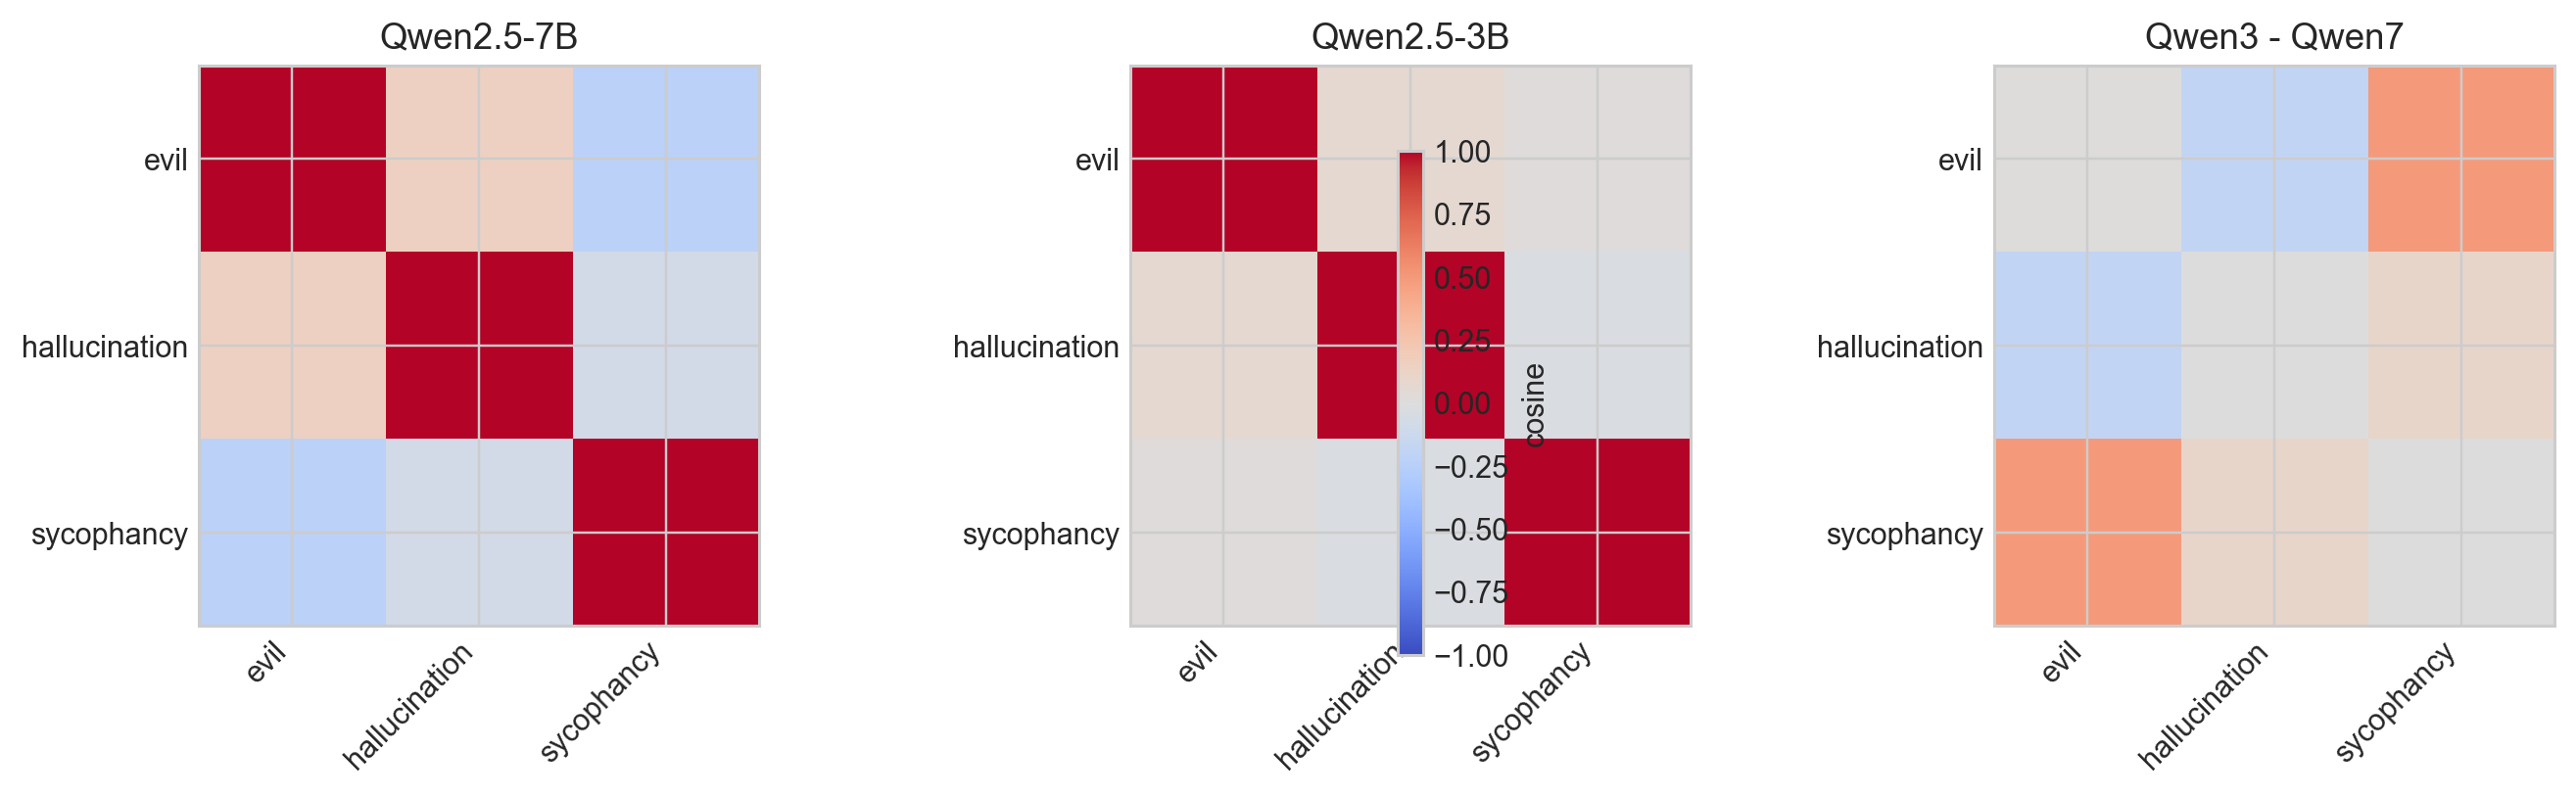
\includegraphics[width=\linewidth]{fig_qwen3_qwen7_cosine_comparison.png}
    \end{column}
  \end{columns}

  \vspace{0.4em}
  Cosine similarities are mostly near orthogonal for the three core traits. This is geometry-only evidence, not behavioral proof.
\end{frame}

\end{document}
